\documentclass[conference, letterpaper]{IEEEtran}

\ifCLASSINFOpdf
   \usepackage[pdftex]{graphicx}
\else
\fi

\usepackage[cmex10]{amsmath}
\usepackage{amssymb}
\usepackage{color}
\usepackage{fancyhdr}
\usepackage[caption=false, font=footnotesize]{subfig}
\usepackage{booktabs}
\usepackage{array}
\usepackage{tabularx}
\newcolumntype{C}{>{\centering\arraybackslash}X}
\usepackage{url}
\usepackage{orcidlink}
\usepackage{threeparttable}
\usepackage{dblfloatfix}

% Relax float placement so wide (double-column) tables can sit near their text
\setcounter{topnumber}{3}
\setcounter{dbltopnumber}{3}
\renewcommand{\topfraction}{0.95}
\renewcommand{\dbltopfraction}{0.95}
\renewcommand{\textfraction}{0.05}
\renewcommand{\floatpagefraction}{0.85}
\renewcommand{\dblfloatpagefraction}{0.85}

\hyphenation{tu-ber-cu-lo-sis ra-di-o-graph}

\renewcommand{\thispagestyle}[1]{}

\fancypagestyle{plain}{
        \fancyhead{}
        \fancyhead[C]{}
        \fancyfoot{}
        \fancyfoot[C]{}
}
\pagestyle{fancy}

\headheight 20pt
\footskip 20pt

\rhead{}

\setcounter{page}{1}

%Header
\fancyhead[R]{\textit{(IJACSA) International Journal of Advanced Computer Science and Applications, \\ Vol. XXX, No. XXX, 2026}}
\renewcommand{\headrulewidth}{0pt}

%Footer
\fancyfoot[C]{www.ijacsa.thesai.org}
\renewcommand{\footrulewidth}{0.5pt}
\fancyfoot[R]{\thepage \  $|$ P a g e }


\begin{document}

\title{A Workflow Support System for Computer-Aided Tuberculosis Screening from Chest X-Rays}

\IEEEoverridecommandlockouts
\author{\IEEEauthorblockN{Raphael B. Alampay~\orcidlink{0000-0001-7498-8830},
Irish Danielle Morales~\orcidlink{0009-0007-4409-5290},
Ruben A. Saulog~\orcidlink{0009-0001-2103-6032} and
Patricia Angela R. Abu~\orcidlink{0000-0002-8848-6644}}
\IEEEauthorblockA{Department of Information Systems and Computer Science, Ateneo de Manila University, Quezon City, Philippines}}

\maketitle

% ============================================================
% ABSTRACT
% ============================================================
\begin{abstract}
Tuberculosis (TB) causes more deaths than any other infectious disease worldwide. While computer-aided detection (CAD) systems used in TB screening programs achieve high diagnostic accuracy, several practical challenges emerge in the screening workflow. Commercial TB CAD products often do not account for X-ray image quality, post-deployment monitoring, and explanation of findings in natural language for screening teams, which often do not involve a radiologist. We present a prototype workflow support system for TB screening to address these issues. Its lead contribution is a clinically grounded LLM explanation module that describes model findings in natural language, a feature not yet present in the commercial products we reviewed. Supporting modules add an input quality gate to assess X-ray image quality and a post-deployment monitoring dashboard. We also develop and benchmark custom models for TB classification and localization. Our results show that ... (TODO).
% TODO: Add quantitative results summary once evaluation is complete.
\end{abstract}

\begin{IEEEkeywords}
Tuberculosis; Computer-Aided Detection; Chest X-ray; Medical Imaging; Computer Vision 
\end{IEEEkeywords}

\IEEEpeerreviewmaketitle

% ============================================================
% I. INTRODUCTION
% ============================================================
\section{Introduction}

Tuberculosis (TB) causes more deaths than any other infectious disease worldwide~\cite{who_global_tb_2024}. It is caused by airborne \textit{Mycobacterium tuberculosis} and primarily affects the lungs~\cite{pai2016tb}. Low- and middle-income countries bear a disproportionate share of the burden, compounded by limited access to diagnostics, delayed presentation, and overburdened health infrastructure~\cite{who_screening_2021}.

\begin{table*}[!t]
\label{tab:feature_comparison}
\renewcommand{\arraystretch}{1.2}
\centering
\begin{threeparttable}
\caption{Feature Comparison with Commercial TB CAD Products}
\label{tab:product_comparison}
\scriptsize
\setlength{\tabcolsep}{4pt}
\begin{tabularx}{\textwidth}{@{}X *{7}{c}@{}}
\toprule
\textbf{Feature} & \textbf{qXR}~\cite{qxr_docs} & \textbf{CAD4TB+}~\cite{cad4tb_product} & \textbf{Lunit}~\cite{lunit_product} & \textbf{DrAid}~\cite{draid_product} & \textbf{Genki}~\cite{genki_product} & \textbf{InferRead}~\cite{inferread_product} & \textbf{Proposed} \\
\midrule
Chest X-ray quality assessment & & & & \textit{n/a} & \textit{n/a} & & $\checkmark$ \\
Monitoring and analytics dashboard & & & $\checkmark$ & \textit{n/a} & \textit{n/a} & & $\checkmark$ \\
Heatmap/overlay of localization findings & $\checkmark$ & $\checkmark$ & $\checkmark$ & $\checkmark$ & $\checkmark$ & $\checkmark$ & $\checkmark$ \\
Explanation of findings in natural language & & & & \textit{n/a} & \textit{n/a} & & $\checkmark$ \\
\bottomrule
\end{tabularx}
\begin{tablenotes}[flushleft]
\scriptsize
\item $\checkmark$ marks a feature documented as present; blank marks a feature documented as absent or not offered; \textit{n/a} marks features for which no documentation was found.
\item The monitoring/analytics dashboard column denotes a post-deployment dashboard for tracking model usage and performance over time.
\end{tablenotes}
\end{threeparttable}
\end{table*}

TB omputer-aided detection (CAD) systems have matured into routine clinical use. The World Health Organization (WHO) endorsed CAD systems as an alternative to human readers for people aged 15 years and older~\cite{who_cad_policy_2021}. TB screening programs often use mobile X-ray units and CAD systems, where CAD substitutes for human readers~\cite{stoptb_cad_guide}~\cite{find_cad_landscape}. In 2025, WHO approved six commercial products as meeting its TB screening performance standards~\cite{who_cad_approval_2025}. In one reader study, AI-CAD assistance improved radiologist performance and enabled non-radiologists to achieve similar performance as radiologists~\cite{anderson2024deep}. Several reviews report model accuracy approaching WHO targets across populations~\cite{ahmad2023systematic, scott2024tb_cad_africa, khan2025tb_meta}, indicating that the field has moved beyond improving accuracy toward real-world use in high-volume screening programs.

\subsection{Gaps in Screening Workflow Integration}

Reviews and deployment studies consistently identify gaps in practical implementation of CAD systems. Among CXR AI studies, workflow integration, local validation, and human factors remain under-studied~\cite{mongan2023review, ahmad2023systematic}. An India deployment identified barriers in workflow, connectivity, and interpretation~\cite{vijayan2023india_tb_cad}, a Vietnam deployment showed only 47.3\% agreement between physician and CAD interpretations at three months~\cite{innes2023vietnam_tb_cad}, and clinicians across countries valued CAD as a complement rather than a replacement~\cite{creswell2023user_perspectives_tb}. The following gaps emerge in the literature:

\textbf{Image quality varies in real-world use.} Chest X-ray (CXR) is the most widely used modality for TB screening~\cite{burrill2007tb_radiology}. TB CAD systems are trained on curated datasets, but CXR images may be poorly positioned, clipped, underexposed, or photographed from analog film~\cite{desita2026photographed}, especially in community screening programs using mobile X-ray units. Poor input quality degrades performance, yet most systems do not expose user-facing quality assessment before inference~\cite{mongan2023review, degrave2021shortcut}.

\textbf{Heatmaps for explaining model findings lack clinical utility.} All commercial TB CAD products in Table \ref{tab:product_comparison} provide heatmaps for model explainability. However, heatmaps are less intuitive for radiologists than discrete localized findings~\cite{ihongbe2024xai_cxr}, often overlap poorly with expert-identified regions, and do not convey the contextual reasoning used during diagnosis~\cite{chen2022xai_human_centered}. A TB CAD acceptability study found that users wanted to understand why the model reached its conclusions~\cite{hua2025qxr_acceptability}. Textual descriptions and case-based reasoning have been proposed as more clinically meaningful alternatives~\cite{borys2023xai_beyond_saliency, siemens_llm_cxr_2023}.

\textbf{Post-deployment monitoring is often lacking.} Deployed performance may shift due to population, equipment, or software changes~\cite{finlayson2021shift}. The U.S. Food and Drug Administration has identified these as risks to AI-enabled medical devices and initiated research on proactive post-market monitoring~\cite{fda_postmarket}, but in practice this remains an operational gap~\cite{mongan2023review}.

\subsection{Related Work}

Related literature has explored models to explain findings in natural language, although this is not yet implemented in deployed systems or commercial products. In a research prototype, Siemens Healthineers paired a combined classification-localization model~\cite{ghesu2022ssl_medical} with a domain-adapted LLM to generate CXR findings~\cite{siemens_llm_cxr_2023}. General medical vision-language models such as LLaVA-Med~\cite{li2023llava_med} and CXR-LLaVA~\cite{lee2024cxr_llava} demonstrate image-conditioned radiology text generation, and recent surveys catalogue the rapid growth of vision-language models for medical report generation~\cite{bazi2024vlm_review}.

We compare against the six WHO-approved TB CAD products in Table~\ref{tab:product_comparison}: qXR v4.0~\cite{qxr_docs}, CAD4TB v7~\cite{cad4tb_product}, Lunit INSIGHT CXR v3.1~\cite{lunit_product}, DrAid v2.4.4--6~\cite{draid_product}, Genki Edge v3.4.2~\cite{genki_product}, and InferRead DR Chest v1.0.1.1~\cite{inferread_product}~\cite{who_cad_approval_2025}. While all provide heatmap localization, post-deployment monitoring is uncommon, input quality assessment is largely absent, and no product is known to explain findings in natural language.

\subsection{Scope and Contribution}

This paper presents a workflow support system for TB screening that targets the gaps above. Its contributions are:

\begin{enumerate}
    \item A \textbf{natural language explanation module} (lead contribution) that describes detected abnormalities with clinical grounding, supporting bounding box-level visual evidence.
    \item An \textbf{input quality assessment module} that screens CXR images for acquisition defects before inference.
    \item A \textbf{post-deployment monitoring dashboard} tracking system behavior and performance over time.
\end{enumerate}

As a secondary contribution, we develop and benchmark custom models for classification (Section \ref{sec:tb_classification}) and localization  (Section \ref{sec:tb_localization}).

% ============================================================
% II. MATERIALS AND METHODS
% ============================================================
\section{System Overview}

\begin{figure}[!tb]
    \centering
    \includegraphics[width=\linewidth]{../figures/pipeline.png}
    \caption{Overview of the proposed TB CAD pipeline.}
    \label{fig:pipeline}
\end{figure}

Figure \ref{fig:pipeline} describes the system overview. A CXR (DICOM or standard image format) is ingested from the screening unit's X-ray or uploaded directly, then evaluated for acquisition quality. Images passing quality screening are scored by the TB classification module. For images flagged as TB, localization (object detection) is done to detect active and latent TB regions. Findings are passed to a module that generates a natural language description of the findings based in clinical context. Outputs are displayed in the interface, and each case is logged for post-deployment monitoring.

% ============================================================
% INPUT QUALITY ASSESSMENT
% ============================================================
\section{Input Quality Assessment}
\label{sec:iqa}

% The input quality gate evaluates each radiograph before it reaches the classifier. It assigns one of four status labels:

% \begin{itemize}
%     \item \textbf{Acceptable:} meets acquisition criteria and proceeds to classification.
%     \item \textbf{Borderline:} minor quality issues (slight rotation, suboptimal exposure) that may reduce confidence. Classification proceeds with a quality warning attached.
%     \item \textbf{Repeat recommended:} significant defects (clipped lung fields, severe underexposure) likely to compromise reliability. The system recommends re-acquisition.
%     \item \textbf{Manual review required:} non-standard input (photographed analog film, lateral view, non-chest image). The case is routed to human review.
% \end{itemize}

% The gate is a hybrid pipeline combining DICOM header checks, a learned view classifier, and an anatomical-segmentation-based sanity check. Concretely: (i) DICOM tags (\texttt{ViewPosition}, \texttt{BodyPartExamined}, \texttt{PhotometricInterpretation}) are read first; any study with a non-frontal \texttt{ViewPosition} is routed to manual review, and inconsistent \texttt{BodyPartExamined} triggers a rejection. (ii) For cases lacking reliable DICOM headers, a small view classifier trained on frontal / lateral labels from PadChest~\cite{bustos2020padchest} serves as a fallback. (iii) The image is passed through the pretrained anatomical segmentation network from the \texttt{torchxrayvision} library~\cite{cohen2022torchxrayvision}, which produces per-pixel masks for left lung, right lung, heart, and other thoracic structures. The gate computes three summary statistics from these masks: the lung-area-to-image-area ratio (a field-of-view score, flagging clipped fields), the lateral offset of the lung centroid relative to image center (a rotation proxy), and the presence of both lung masks above a minimum area (a non-chest-image check). (iv) Classical image statistics (Laplacian variance for blur; 1st/99th percentile intensity gaps for under- or over-exposure) are thresholded on development data and added to the rule set. The combined rules map each image to one of the four status labels above.

% This design is motivated by evidence that CXR AI performance degrades when applied to images differing from the training distribution. A systematic review of cross-population domain shift found that 81\% of deep learning algorithms in radiology exhibited decreased accuracy on external datasets~\cite{domain_shift_cxr_2025}, and shortcut learning, where models rely on acquisition artifacts rather than pathological features, has been documented as a failure mode in CXR AI~\cite{degrave2021shortcut, mongan2023review}. The gate is engineered rather than novel. It is included as prior art establishing that a clinically adequate CXR screening system has a well-defined acquisition-quality model upstream of inference.

% Local threshold calibration matters for adapting CAD to site-specific prevalence and clinical context. WHO has published calibration guidance~\cite{who_calibration}, and CAD4TB+ offers dynamic threshold adjustment~\cite{cad4tb_product}. A 2025 triage study demonstrated the sensitivity-specificity tradeoff from threshold selection~\cite{marquez2025philippines}. The classifier operating point is therefore retained as a configurable parameter, but it is not a headline contribution. It addresses a partially solved problem for which guidance already exists.

% \subsection{Results}

% TODO: Report input-quality-gate accuracy, status-label distribution, and rejection-rate analysis.

% ============================================================
% TUBERCULOSIS CLASSIFICATION
% ============================================================
\section{Tuberculosis Classification}
\label{sec:tb_classification}

The TB classification module flags each CXR as either healthy, sick non-TB, or TB as seen in Figure~\ref{fig:pipeline}.

\begin{table*}[!t]
\renewcommand{\arraystretch}{1.2}
\centering
\begin{threeparttable}
\caption{Tuberculosis Classification Results}
\label{tab:classification_results}
\small
\begin{tabular}{@{}l c c c c c c c c@{}}
\toprule
\textbf{Model} & \textbf{AUC$_{\text{TB}}$} & \textbf{Acc. (\%)} & \textbf{Sens. (\%)} & \textbf{Spec. (\%)} & \textbf{Avg. Prec. (\%)} & \textbf{Avg. Rec. (\%)} & \textbf{Avg. F1 (\%)} & \textbf{Params} \\
\midrule
FlipR                  & 0.9984 & 98.97 & 94.17 & \textbf{99.91} & \textbf{99.01} & 97.70 & 98.34 & \textbf{2.8M} \\
EfficientNet-B0        & \textbf{0.9995} & 98.89 & 95.00 & 99.65 & 98.29 & 97.87 & 98.07 & 5.3M \\
MobileNetV3-Large      & \textbf{0.9995} & \textbf{99.21} & \textbf{96.67} & 99.82 & 98.97 & \textbf{98.54} & \textbf{98.75} & 5.5M \\
Drax-MobileNetV3-Large & 0.9989 & 98.81 & 95.00 & 99.65 & 98.23 & 97.81 & 98.02 & 6.1M \\
DenseNet-121           & 0.9975 & 98.57 & 92.50 & 99.56 & 97.81 & 96.97 & 97.38 & 8.0M \\
ResNet-18              & 0.9982 & 98.17 & 93.33 & 99.21 & 96.71 & 96.90 & 96.80 & 11.7M \\
DraxNet                & 0.9988 & 98.41 & 95.00 & 99.47 & 97.51 & 97.51 & 97.51 & 17.0M \\
ResNet-50              & 0.9978 & 97.70 & 92.50 & 99.47 & 96.95 & 96.33 & 96.63 & 25.6M \\
ConvNeXt-Tiny          & 0.9952 & 97.14 & 95.00 & 97.98 & 93.63 & 96.58 & 94.97 & 28.6M \\
\bottomrule
\end{tabular}
\begin{tablenotes}[flushleft]
\footnotesize
\item AUC$_{\text{TB}}$ is the area under the ROC curve for the TB class. Sensitivity is recall for the TB class. Specificity is recall for the non-TB class (healthy and sick non-TB combined). Precision, recall, and F1 are averaged across the three classes (healthy, sick non-TB, TB).
\end{tablenotes}
\end{threeparttable}
\end{table*}

\subsection{Dataset}

Classification and localization models are trained on TBX11K~\cite{liu2020tbx11k}, a public CXR dataset with image-level labels (\textit{healthy}, \textit{sick non-TB}, \textit{TB}) and bounding-box-level labels (\textit{active-TB}, \textit{latent-TB}). We use a simplified redistribution\footnote{\url{https://www.kaggle.com/datasets/vbookshelf/tbx11k-simplified}} with 8,400 CXRs (3,800 healthy, 3,800 sick non-TB, 800 TB), with a 79\%/21\% train/validation split (6,600 and 1,800 images). TBX11K is selected since it is the largest public TB CXR dataset combining a TB-specific sample large enough to train from scratch, expert bounding-box annotations, a sick non-TB class, and a demographic and class composition that reflect real-world clinical settings~\cite{liu2023tbx11k_pami}.

The official TBX11K test set is withheld for an online challenge, so we evaluate on the public validation set. Our results are therefore not directly comparable to SymFormer~\cite{liu2023tbx11k_pami} or other challenge entries on the private test set.

\subsection{Data Preprocessing}

Classification models are trained without preprocessing or data augmentation. CXRs unfit for inference are already filtered out by the input quality assessment module. CXRs are also acquired under a standardized posteroanterior protocol and are largely uniform in pose, so aggressive augmentation risks introducing distribution shift.

\subsection{Model Architecture}

We evaluate nine classifiers: six baselines (EfficientNet-B0~\cite{tan2019efficientnet}, MobileNetV3-Large~\cite{howard2019mobilenetv3}, DenseNet-121~\cite{huang2017densenet}, ResNet-18, ResNet-50~\cite{he2016resnet}, ConvNeXt-Tiny~\cite{liu2022convnext}) and three custom models (DraxNet, Drax-MobileNetV3-Large, FlipR).

\subsubsection{DraxNet}

DraxNet ($17.0$M parameters) modifies a ResNet-18 backbone so the fourth layer consists of two ResNet blocks, each with a custom mixer (\emph{DraxBlock}) inserted between its two convolutions. All other components are unchanged. \emph{DraxBlock} consists of a ConvNeXt local convolutional branch followed by an optional self-attention branch, fused via stochastic-depth residuals. DraxNet, short for Dynamic Residual Attention eXchange, reserves the heavier mixer for the final, lowest-resolution stage, adding attention capacity with fewer parameters than a full attention backbone.

\subsubsection{Drax-MobileNetV3-Large}

Drax-MobileNetV3-Large ($6.1$M parameters) applies the DraxBlock to a parameter-efficient backbone. The MobileNetV3-Large feature extractor and head are unchanged, and a bottlenecked \emph{DraxBlock} is inserted after the final feature stage. This tests whether the DraxBlock generalizes beyond a ResNet-style backbone.

\subsubsection{FlipR}

FlipR ($2.8$M parameters) inserts a \emph{FlipR} block between layers of an otherwise unchanged ResNet-18. The \emph{FlipR} block computes the difference between each feature map and its horizontally flipped counterpart, smoothed by average pooling to account for imperfect anatomical symmetry, then broadcasts a gated mask across all channels. The block is inspired by SymAttention~\cite{liu2023tbx11k_pami}, which observes that bilateral asymmetry in CXRs is a key indicator of TB. FlipR tests whether a lightweight symmetry gate can match heavier attention approaches.

\subsection{Model Training}

All models are trained from scratch with a fixed random seed, batch size $16$, $512\times512$ input, $100$ epochs, Adam at a fixed learning rate of $10^{-3}$, no schedule, and unweighted cross-entropy loss. No hyperparameter tuning was done.

\subsection{Results}

Classification results are reported in Table~\ref{tab:classification_results}.

\textbf{MobileNetV3-Large is the top classifier, while FlipR achieves comparable results with half the parameters.} Given the small ($\pm 1\%$) differences, ordering among the top four (FlipR, EfficientNet, MobileNetV3-Large, Drax-MobileNetV3-Large) is likely due to stochasticity. They differ most on sensitivity ($\pm 2.5\%$), so we interpret MobileNetV3-Large ($96.67\%$ sensitivity) as the top model, since sensitivity is the clinically dominant metric in TB screening. FlipR reaches comparable results on other metrics at roughly half the size ($2.8$M vs $5.5$M), supporting the SymFormer~\cite{liu2023tbx11k_pami} hypothesis that bilateral asymmetry is highly indicative of TB.

\textbf{All models meet WHO targets for TB triage.}
Sensitivity ranges from $92.50$ to $96.67\%$, clearing the WHO target of $90\%$ sensitivity. Specificity ranges from $97.98$ to $99.91\%$, well above the WHO target of $70\%$ specificity~\cite{who_screening_2021}. Sensitivity is more clinically important than specificity in screening, since a missed TB case risks untreated transmission while a false positive triggers only confirmatory testing. The top model, MobileNetV3-Large, misses only $3.3\%$ of TB cases.

\textbf{The high-specificity, lower-sensitivity profile is likely attributable to TBX11K rather than model architecture.}
Models in the literature consistently show the same pattern on TBX11K. The dataset is constructed to reward high specificity, since the common failure mode on other TB datasets is over-predicting TB and collapsing specificity to near-zero~\cite{liu2023tbx11k_pami}.

\textbf{Lightweight models are preferred for TB screening on both performance and deployment grounds.}
Smaller models outperform larger ones across the board: MobileNetV3-Large ($5.5$M), EfficientNet-B0 ($5.3$M), and FlipR ($2.8$M) beat all larger models in accuracy and F1. Due to a modest TBX11K training set, a minority TB class, and no class-imbalance handling, larger networks appear to overfit the majority healthy and sick non-TB classes rather than learn discriminative TB features. TB screening also runs in resource-limited settings often without a dedicated GPU, so a lightweight model is preferable in deployment.

% ============================================================
% TUBERCULOSIS LOCALIZATION
% ============================================================
\section{Tuberculosis Localization}
\label{sec:tb_localization}

\subsection{Dataset}

Localization uses the TBX11K bounding-box annotations, with each region labeled active TB or latent TB~\cite{liu2020tbx11k}. Active TB denotes ongoing, transmissible infection requiring treatment; latent TB denotes prior, inactive infection that is not contagious but may reactivate. As Figure~\ref{fig:pipeline} shows, active TB is more visually salient and latent TB is more subtle. A TB-labeled CXR may contain only active-TB lesions ($924$ images), only latent-TB lesions ($212$ images), or both ($54$ images), a composition consistent with real-world conditions.

\subsection{Model Architecture}

We evaluate YOLO26 and a custom variant in which the detector's default feature extractor is replaced by the DraxNet backbone used in classification. The detection head and training protocol are unchanged, isolating the backbone's effect on localization.

\subsection{Model Training}

Localization uses the same training configuration as the classification models (Section~\ref{sec:tb_classification}).

\begin{table}[!ht]
\renewcommand{\arraystretch}{1.2}
\centering
\begin{threeparttable}
\caption{Tuberculosis Localization Results}
\label{tab:detection_results}
\small
\begin{tabular}{@{}l l c c@{}}
\toprule
\textbf{Model} & \textbf{Class} & \textbf{mAP$_{50}$} & \textbf{mAP$_{50\text{-}95}$} \\
\midrule
YOLO26                    & ATB & 0.4511 & 0.2110 \\
YOLO26                    & LTB & \textbf{0.1070} & \textbf{0.0410} \\
\midrule
YOLO26 + DraxNet & ATB & \textbf{0.5865} & \textbf{0.2748} \\
YOLO26 + DraxNet & LTB & 0.1017 & 0.0310 \\
\bottomrule
\end{tabular}
\begin{tablenotes}[flushleft]
\footnotesize
\item ATB = active TB; LTB = latent TB.
\end{tablenotes}
\end{threeparttable}
\end{table}

\subsection{Results}

\begin{figure}[!t]
\centering
\subfloat{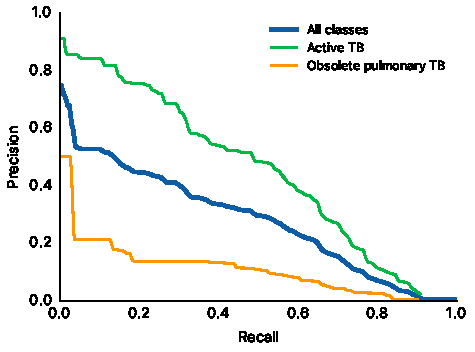
\includegraphics[width=0.48\columnwidth]{../figures/pr_yolo26.pdf}}
\hfil
\subfloat{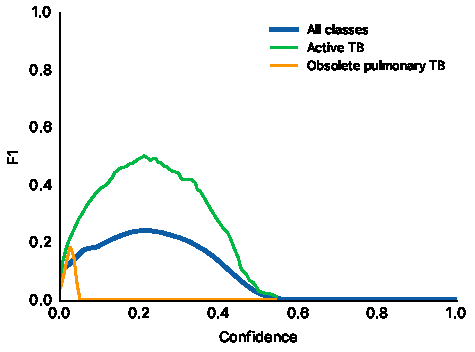
\includegraphics[width=0.48\columnwidth]{../figures/f1_yolo26.pdf}}
\\
\subfloat{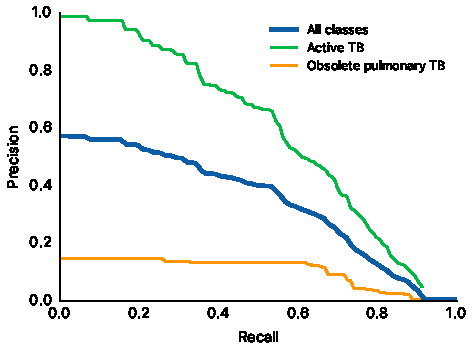
\includegraphics[width=0.48\columnwidth]{../figures/pr_draxnet.pdf}}
\hfil
\subfloat{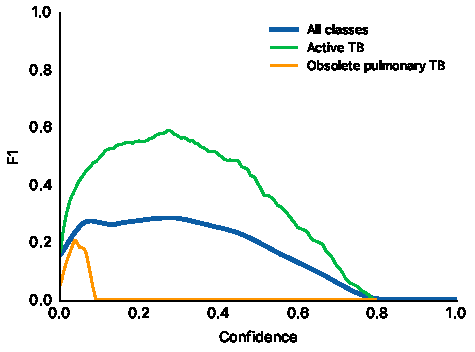
\includegraphics[width=0.48\columnwidth]{../figures/f1_draxnet.pdf}}
\caption{Localization precision-recall (left) and F1-confidence (right) curves for YOLO26 (top) and YOLO26 with the DraxNet backbone (bottom). Both sustain high precision while recall saturates near $0.26$, and the latent-TB curve collapses at low confidence, so localization functions as a high-precision rule-in cue rather than a standalone detector.}
\label{fig:detection_curves}
\end{figure}

Localization results per class are reported in Table~\ref{tab:detection_results}.

% TODO: evidence
% \textbf{DraxNet improves on the locations of detected active TB regions, but does not detect more regions overall.}

\textbf{Active TB is more likely to be detected than latent TB.}
Both detectors localize active TB roughly four times more accurately than latent TB at $\mathrm{mAP}_{50}$ and roughly five to nine times more accurately at $\mathrm{mAP}_{50\text{-}95}$. This gap reflects the TBX11K class imbalance (active-TB regions outnumber latent-TB regions roughly 4:1) and the subtle appearance of latent-TB lesions. The TBX11K reference reports the same pattern across all detection methods, attributing it to imbalance~\cite{liu2023tbx11k_pami}, and it is consistent with human readers distinguishing latent TB less reliably~\cite{choi2023tb_activity}. The bias toward active TB also aligns with clinical triage priorities, since active TB requires urgent treatment.

\textbf{The DraxNet backbone specializes toward active TB.}
YOLO26 with the DraxNet backbone raises active-TB $\mathrm{mAP}_{50}$ from $0.4511$ to $0.5865$ ($+0.1354$) and $\mathrm{mAP}_{50\text{-}95}$ from $0.2110$ to $0.2748$ ($+0.0638$), while slightly reducing latent-TB ($0.1070 \rightarrow 0.1017$ at $\mathrm{mAP}_{50}$; $0.0410 \rightarrow 0.0310$ at $\mathrm{mAP}_{50\text{-}95}$). The gain is driven almost entirely by precision ($0.74 \rightarrow 0.82$). Recall is unchanged at roughly $0.26$.

\textbf{Recall, not precision, is the bottleneck.}
Both detectors localize confidently but find only about a quarter of the annotated TB regions. Figure~\ref{fig:detection_curves} shows precision staying high while recall saturates near $0.26$, and the latent-TB curve collapsing at low confidence for both detectors.

\textbf{Localization is useful to confirm (rule-in) TB, but not to rule it out.} The high-precision, low-recall profile dictates clinical use: a flagged lesion is likely correct and warrants focused radiologist review, but the detector must not exclude TB since most annotated lesions are missed. Localization is therefore most reliable as supporting region-level evidence for the classifier and LLM explanation modules, rather than as a standalone detector.

% ============================================================
% MULTIMODAL EXPLANATION
% ============================================================
\section{Multimodal Explanation}
\label{sec:explanation}

% The multimodal explanation module is the lead contribution. It translates the classifier's evidence into a natural-language statement that a clinician can read, understand, and act on without interpreting heatmaps or understanding the model's internals. Evidence for the value of natural-language explanation in CXR AI comes from user studies and clinician-interview research, though the demand picture is mixed. In a user-centered evaluation of explainability techniques on chest radiographs with 26 clinicians at a National Health Service trust in the United Kingdom, a majority stated that descriptive sentences should be added alongside visual explanations, and roughly half reported that colored heatmap overlays hindered readability~\cite{ihongbe2024xai_cxr}. A multisite prospective study of 220 physicians reading chest radiographs found that the form of AI explanation materially affected diagnostic performance and physician trust, indicating that explanation modality, not only the presence of an explanation, shapes clinical use~\cite{gaube2024care_explain}. Broader interview-based studies of AI decision support in medicine have surfaced consistent requests for contextual reasoning and explanatory information rather than predictions alone~\cite{tonekaboni2019clinicians_want, cai2019hello_ai}. In the TB CAD setting specifically, a qualitative study of radiologists using a commercial TB CXR product found opinion divided: one participant reported struggling to understand why the system reached a given conclusion, while another characterized the tool as an engine whose internal workings were not clinically relevant to them~\cite{hua2025qxr_acceptability}. The module is therefore positioned as most useful for a radiologist-in-the-loop or confirmatory reader reviewing flagged cases, rather than as a universally demanded feature for frontline screeners who primarily act on the abnormality score.

% Given a radiograph and the classifier's output, the module generates a statement identifying the suspected finding (for example, a cavitary lesion, upper-lobe infiltrate, or pleural effusion), its anatomical location (for example, the right upper lobe or left costophrenic angle), and a clinical reasoning link connecting the finding to the TB classification. An example output: \textit{``TB suspected. The model identified an area of increased opacity in the right upper lobe consistent with an infiltrate. Upper-lobe infiltrates are among the most common radiographic findings in active pulmonary tuberculosis.''} This differs from heatmap-only explanations in two ways. First, it names the finding in clinical vocabulary rather than highlighting a region. Second, it provides a reason, grounded in radiographic knowledge, for why that finding supports a TB classification.

% ============================================================
% STRUCTURED EVIDENCE INTERFACE
% ============================================================
\section{Structured Evidence Interface}
\label{sec:interface}

% All outputs are consolidated into a single panel for rapid clinical review: the TB probability score as a numeric value and color-coded risk band (low, moderate, high); the quality status with warnings for detected issues; a heatmap overlay showing regions influencing the prediction; and the natural-language explanation from the multimodal module. The panel uses a traffic-light color scheme for risk and quality status and is designed to be reviewable in under 30 seconds during routine triage.
% TODO: Include interface mockup or screenshot (Figure 2).

% ============================================================
% POST-DEPLOYMENT MONITORING
% ============================================================
\section{Post-Deployment Monitoring}
\label{sec:monitoring}

% A monitoring dashboard tracks operational metrics to detect behavioral changes after deployment, drawing on the literature on post-deployment medical-AI monitoring~\cite{finlayson2021shift, feng2022continual, merkow2024drift, rudolph2024postdeploy_cxr} and metrics published by existing TB CAD products~\cite{qxr_docs, cad4tb_product, lunit_product}. Metrics are organized into five groups: input-side (case volume, quality-gate rejection rate, scanner/site/demographic mix relative to training); prediction-side (TB-score distribution, flag rate, per-finding trajectory, calibration metrics); outcome-side (radiologist override rate, CAD-human discordance, and bacteriologically confirmed TB yield among CAD-positive cases, explicitly called for in WHO guidance~\cite{who_screening_2021}); drift (Population Stability Index and Kolmogorov--Smirnov statistics on score distributions, with PSI $<0.1$ stable, $0.1$--$0.25$ flagged, $\geq 0.25$ a major shift~\cite{feng2022continual}, plus higher-dimensional embedding drift detection~\cite{merkow2024drift, ghosh2024drift}); and fairness (sensitivity, specificity, and positive predictive value stratified by clinically relevant subgroups with per-subgroup confidence intervals, as required by regulatory guidance~\cite{fda_postmarket}). The dashboard does not autonomously adjust system behavior. It enables human intervention when metrics indicate degradation or drift~\cite{mongan2023review, rudolph2024postdeploy_cxr}.

% ============================================================
% DISCUSSION
% ============================================================
\section{Discussion}

% The modules form a single screening workflow rather than a set of independent models. The classification and localization experiments suggest that compact custom backbones can match or exceed standard ResNet baselines on TBX11K, while the explanation, interface, and monitoring components target the laboratory-to-deployment gaps identified in the Introduction. The intended contribution is integrative: each module is individually modest, but their composition addresses needs that detection accuracy alone does not. These claims are preliminary. The evaluation reported here is partial, and the end-to-end workflow argument is made rather than yet demonstrated in a clinical setting.

\subsection{Limitations}

% This work has several limitations. First, the system has not been evaluated in a live clinical environment. Evaluation relies on retrospective data and simulated workflows. Second, the explanation module's outputs have not been validated against expert radiologist interpretations at scale, and incorrect explanations could reduce rather than build trust. Third, quality gate thresholds were set on development data and may require recalibration for different imaging environments. Fourth, the TB detection module processes only a single frontal (posteroanterior or anteroposterior) chest radiograph per case, a constraint shared by all WHO-approved TB CAD products, which are trained exclusively on frontal projections. Unlike a clinical PACS hanging protocol that presents current and prior images side by side, the system cannot compare serial radiographs. This restricts its use to screening of new patients at a single time point. It cannot track radiographic change over the course of TB treatment or detect progression and regression across follow-up examinations. Fifth, all model evaluation uses a single dataset, the public simplified split of TBX11K, with the official multi-class test set withheld behind an online challenge. Generalization to other patient populations, scanners, acquisition conditions, and to the official four-class TBX11K benchmark is therefore unverified and would require external validation. The reported model results also include several explicit negative findings, stated rather than omitted: latent (obsolete) TB is localized poorly, overall detection recall is low, the deeper ResNet-50 underperforms the smaller ResNet-18 on TB sensitivity, and the FlipR run did not complete. Finally, the multimodal explanation module is a prototype, not a clinically validated explanation system: the grounding-by-construction approach reduces but does not eliminate error, since templated sentences can still propagate incorrect detector outputs and the LLM smoothing step could paraphrase findings in ways that shift clinical meaning, which is why the post-hoc verification step is included.

\subsection{Future Work}

% \begin{itemize}
%     \item \textbf{Prospective clinical evaluation.} Hospital deployment with measurement of diagnostic outcomes, clinician behavior, and patient impact.
%     \item \textbf{Cost-effectiveness analysis.} Assessment of whether the clinical workflow integration layer reduces unnecessary testing, missed cases, or clinical time. Cost data for AI-CAD workflows in high-burden settings are fragmented. A local pilot study would be needed to produce credible estimates.
%     \item \textbf{Photographed-film workflows.} Extension of the quality gate to handle smartphone-captured analog radiographs, common in rural health facilities in high-burden countries, with dedicated evaluation of domain shift~\cite{nasser2023photographed}.
%     \item \textbf{Formal explanation validation.} Systematic comparison of generated explanations against radiologist reports.
%     \item \textbf{Trainee-oriented evaluation.} Primary user research with residents and non-radiologist physicians to determine whether a dedicated trainee mode is actually demanded, what form it should take, and whether it produces durable skill gains rather than in-session dependence.
% \end{itemize}

% ============================================================
% CONCLUSION
% ============================================================
\section{Conclusion}

% TB CAD classifiers are now accurate enough for screening. The open problem is making their outputs safe, interpretable, and usable in hospital workflows. This paper presented a prototype clinical workflow integration layer that wraps a mature TB CAD backbone with a clinically grounded multimodal explanation module, an input quality gate, a structured evidence interface, and a post-deployment monitoring dashboard. A full evaluation of feasibility and clinical utility is left to future work.

% TODO: Finalize once results and full discussion are available.
% Frame as: the field has moved from "can TB CAD classify chest X-rays?"
% to "how can a prototype integrate clinical workflow support and clinician-facing
% explanation around mature TB CAD for hospital use?"

% ============================================================
% ACKNOWLEDGMENTS
% ============================================================
\section*{Acknowledgments}

The authors would like to thank the University Research Council (URC) of Ateneo de Manila University for supporting this work through a URC Standard Grant (URC 2025-20).

% ============================================================
% DECLARATION ON GENERATIVE AI
% ============================================================
\section*{Declaration on Generative AI}

Generative AI tools were used to assist in drafting and preparing this manuscript. The conception of the research, methodology, and conclusions are the work of the authors.

% ============================================================
% REFERENCES
% ============================================================
\begin{thebibliography}{40}

\bibitem{who_global_tb_2024}
World Health Organization, ``Global Tuberculosis Report 2024,'' Geneva: WHO, 2024. [Online]. Available: https://www.who.int/teams/global-tuberculosis-programme/tb-reports/global-tuberculosis-report-2024

\bibitem{who_screening_2021}
World Health Organization, ``WHO consolidated guidelines on tuberculosis. Module 2: Screening -- Systematic screening for tuberculosis disease,'' Geneva: WHO, 2021. [Online]. Available: https://www.who.int/publications/i/item/9789240022676

\bibitem{pai2016tb}
M. Pai, M. A. Behr, D. Dowdy, K. Dheda, M. Divangahi, C. C. Boehme, A. Ginsberg, S. Swaminathan, M. Spigelman, H. Getahun, D. Menzies, and M. Raviglione, ``Tuberculosis,'' \emph{Nature Reviews Disease Primers}, vol. 2, art. 16076, 2016, doi: 10.1038/nrdp.2016.76.

\bibitem{burrill2007tb_radiology}
J. Burrill, C. J. Williams, G. Bain, G. Conder, A. L. Hine, and R. R. Misra, ``Tuberculosis: A radiologic review,'' \emph{RadioGraphics}, vol. 27, no. 5, pp. 1255--1273, 2007, doi: 10.1148/rg.275065176.

\bibitem{choi2023tb_activity}
Y.~R.~Choi, S.~H.~Yoon, J.~Kim, J.~Y.~Yoo, H.~Kim, and K.~N.~Jin, ``Chest radiography of tuberculosis: determination of activity using deep learning algorithm,'' \textit{Tuberculosis and Respiratory Diseases}, vol.~86, no.~3, pp.~226--233, 2023, doi: 10.4046/trd.2023.0020.

\bibitem{who_cad_policy_2021}
World Health Organization, ``WHO operational handbook on tuberculosis. Module 2: Screening,'' Geneva: WHO, 2021. [Online]. Available: https://www.who.int/publications/i/item/9789240110373

\bibitem{who_cad_approval_2025}
World Health Organization, ``Use of computer-aided detection software for tuberculosis screening: WHO policy statement,'' Geneva: WHO, 2025. [Online]. Available: https://www.who.int/publications/i/item/9789240110373

\bibitem{ahmad2023systematic}
H.~K.~Ahmad \textit{et al.}, ``Machine learning augmented interpretation of chest X-rays: A systematic review,'' \textit{Diagnostics}, vol.~13, no.~4, art.~743, 2023. [Online]. Available: https://pmc.ncbi.nlm.nih.gov/articles/PMC9955112/

\bibitem{anderson2024deep}
P.~G.~Anderson \textit{et al.}, ``Deep learning improves physician accuracy in the comprehensive detection of abnormalities on chest X-rays,'' \textit{Scientific Reports}, vol.~14, 2024. [Online]. Available: https://www.nature.com/articles/s41598-024-76608-2

\bibitem{mongan2023review}
J.~Mongan \textit{et al.}, ``Artificial intelligence and machine learning for chest radiography,'' \textit{Radiology}, vol.~307, no.~3, 2023. [Online]. Available: https://pmc.ncbi.nlm.nih.gov/articles/PMC10128969/

\bibitem{degrave2021shortcut}
A.~J.~DeGrave, J.~D.~Janizek, and S.-I.~Lee, ``AI for radiographic COVID-19 detection selects shortcuts over signal,'' \textit{Nature Machine Intelligence}, vol.~3, pp.~610--619, 2021. [Online]. Available: https://pmc.ncbi.nlm.nih.gov/articles/PMC10047562/

\bibitem{siemens_llm_cxr_2023}
M.~D.~Danu, G.~Marica, S.~K.~Karn, B.~Georgescu, A.~Mansoor, F.~Ghesu, L.~M.~Itu, C.~Suciu, S.~Grbic, O.~Farri, and D.~Comaniciu, ``Generation of radiology findings in chest X-ray by leveraging collaborative knowledge,'' \textit{Procedia Computer Science (ITQM 2023)}, 2023. [Online]. Available: https://arxiv.org/abs/2306.10448

\bibitem{ghesu2022ssl_medical}
F.~C.~Ghesu, B.~Georgescu, A.~Mansoor, Y.~Yoo, D.~Neumann, P.~Patel, R.~S.~Vishwanath, J.~M.~Balter, Y.~Cao, S.~Grbic, and D.~Comaniciu, ``Self-supervised learning from 100 million medical images,'' \textit{arXiv preprint arXiv:2201.01283}, 2022. [Online]. Available: https://arxiv.org/abs/2201.01283

\bibitem{li2023llava_med}
C.~Li \textit{et al.}, ``LLaVA-Med: Training a large language-and-vision assistant for biomedicine in one day,'' \textit{Advances in Neural Information Processing Systems}, 2023. [Online]. Available: https://arxiv.org/abs/2306.00890

\bibitem{lakhani2017deep}
P.~Lakhani and B.~Sundaram, ``Deep learning at chest radiography: Automated classification of pulmonary tuberculosis by using convolutional neural networks,'' \textit{Radiology}, vol.~284, no.~2, pp.~574--582, 2017.

\bibitem{pasa2019efficient}
F.~Pasa \textit{et al.}, ``Efficient deep network architectures for fast chest X-ray tuberculosis screening and visualization,'' \textit{Scientific Reports}, vol.~9, 2019.

\bibitem{who_calibration}
WHO Kobe Centre, ``Determining the local calibration of computer-assisted detection (CAD) thresholds and other parameters.'' [Online]. Available: https://wkc.who.int/resources/publications/i/item/determining-the-local-calibration-of-computer-assisted-detection-(cad)-thresholds-and-other-parameters

\bibitem{marquez2025philippines}
A.~Marquez \textit{et al.}, ``Performance of chest X-ray with computer-aided detection as a triage test for pulmonary TB in the Philippines,'' \textit{BMC Global and Public Health}, 2025. [Online]. Available: https://bmcglobalpublichealth.biomedcentral.com/articles/10.1186/s44263-025-00198-y

\bibitem{qxr_docs}
Qure.ai, ``qXR documentation.'' [Online]. Available: https://documentation.qure.ai/

\bibitem{cad4tb_product}
Delft Imaging, ``CAD4TB+.'' [Online]. Available: https://delft.care/cad4tb/

\bibitem{lunit_product}
Lunit, ``INSIGHT CXR.'' [Online]. Available: https://www.lunit.io/en/products/cxr

\bibitem{draid_product}
VinBrain, ``DrAid for TB screening.'' [Online]. Available: https://draid.ai/

\bibitem{genki_product}
DeepTek, ``Genki: AI for tuberculosis screening.'' [Online]. Available: https://www.deeptek.ai/genki

\bibitem{inferread_product}
Infervision, ``InferRead DR Chest: instruction for use,'' (hosted on the Stop TB Partnership Digital Health Technology Hub). [Online]. Available: https://stoptb.org/assets/documents/dhthub/User\%20Manual\%20Software\%20-\%20InferRead\%20DR\%20Chest.pdf

\bibitem{stoptb_cad_guide}
Stop TB Partnership, ``Screening and triage for TB using computer-aided detection (CAD) technology and ultra-portable X-ray systems: A practical guide,'' Geneva, Switzerland, 2021. [Online]. Available: \url{https://www.stoptb.org/sites/default/files/imported/page/Screening_and_Triage_for_TB_using_Computer-Aided_Detection__CAD__Technology_and_Ultra-portable_X-Ray_Systems-A_Practical_Guide_.pdf}

\bibitem{find_cad_landscape}
FIND, ``Digital chest radiography and computer-aided detection (CAD) solutions for tuberculosis diagnostics: Technology landscape analysis,'' Geneva, Switzerland, 2021. [Online]. Available: \url{https://www.finddx.org/wp-content/uploads/2023/02/20210401_technology_landscape_computer_aided_tb_FV_EN.pdf}


\bibitem{desita2026photographed}
Z.~Desita, T.~Tadesse, A.~S.~Bohlbro \textit{et al.}, ``Computer-aided analysis of photographed chest X-ray films performs well compared with trained radiologists,'' \textit{Mayo Clinic Proceedings: Digital Health}, 2026. [Online]. Available: https://pmc.ncbi.nlm.nih.gov/articles/PMC12955127/

\bibitem{chen2022xai_human_centered}
H.~Chen, C.~Gomez, C.-M.~Huang, and M.~Unberath, ``Explainable medical imaging AI needs human-centered design: guidelines and evidence from a systematic review,'' \textit{npj Digital Medicine}, vol.~5, no.~156, 2022. [Online]. Available: https://www.nature.com/articles/s41746-022-00699-2

\bibitem{borys2023xai_beyond_saliency}
K.~Borys, Y.~A.~Schmitt, M.~Nauta, C.~Seifert, N.~Kr\"{a}mer, C.~M.~Friedrich, and F.~Nensa, ``Explainable AI in medical imaging: An overview for clinical practitioners -- Beyond saliency-based XAI approaches,'' \textit{European Journal of Radiology}, vol.~162, art.~110786, 2023. [Online]. Available: https://doi.org/10.1016/j.ejrad.2023.110786

\bibitem{lee2024cxr_llava}
S.~Lee, J.~Youn, H.~Kim, M.~Kim, and S.~H.~Yoon, ``CXR-LLaVA: a multimodal large language model for interpreting chest X-ray images,'' \textit{European Radiology}, vol.~35, 2025. [Online]. Available: https://link.springer.com/article/10.1007/s00330-024-11339-6

\bibitem{bazi2024vlm_review}
I.~Hartsock and G.~Rasool, ``Vision-language models for medical report generation and visual question answering: a review,'' \textit{Frontiers in Artificial Intelligence}, vol.~7, art.~1430984, 2024. [Online]. Available: https://pmc.ncbi.nlm.nih.gov/articles/PMC11611889/

\bibitem{fda_postmarket}
U.S. Food and Drug Administration, ``Methods and tools for effective postmarket monitoring of artificial intelligence (AI)-enabled medical devices,'' 2024. [Online]. Available: https://www.fda.gov/medical-devices/medical-device-regulatory-science-research-programs-conducted-osel/methods-and-tools-effective-postmarket-monitoring-artificial-intelligence-ai-enabled-medical-devices

\bibitem{rudolph2024postdeploy_cxr}
J.~Rudolph \textit{et al.}, ``Post-deployment performance of a deep learning algorithm for normal and abnormal chest X-ray classification: A study at visa screening centers in the United Arab Emirates,'' \textit{PLOS ONE}, 2024. [Online]. Available: https://pmc.ncbi.nlm.nih.gov/articles/PMC11539241/

\bibitem{chaves2023ai_radiology_education}
A.~S.~Tejani, H.~Elhalawani, L.~Moy, M.~Kohli, and C.~E.~Kahn~Jr, ``Artificial intelligence and radiology education,'' \textit{Radiology: Artificial Intelligence}, vol.~5, no.~1, e220084, 2023. [Online]. Available: https://pubs.rsna.org/doi/full/10.1148/ryai.220084

\bibitem{mazurowski2019ai_precision_education}
M.~A.~Mazurowski, ``Artificial intelligence for precision education in radiology,'' \textit{British Journal of Radiology}, vol.~92, no.~1103, 2019. [Online]. Available: https://pmc.ncbi.nlm.nih.gov/articles/PMC6849670/

\bibitem{vijayan2023india_tb_cad}
S.~Vijayan \textit{et al.}, ``Implementing a chest X-ray artificial intelligence tool to enhance tuberculosis screening in India: Lessons learned,'' \textit{PLOS Digital Health}, vol.~2, no.~12, e0000404, 2023. [Online]. Available: https://journals.plos.org/digitalhealth/article?id=10.1371/journal.pdig.0000404

\bibitem{innes2023vietnam_tb_cad}
A.~L.~Innes \textit{et al.}, ``Computer-aided detection for chest radiography to improve the quality of tuberculosis diagnosis in Vietnam's district health facilities: An implementation study,'' \textit{Tropical Medicine and Infectious Disease}, vol.~8, no.~11, art.~488, 2023. [Online]. Available: https://doi.org/10.3390/tropicalmed8110488

\bibitem{creswell2023user_perspectives_tb}
J.~Creswell \textit{et al.}, ``Early user perspectives on using computer-aided detection software for interpreting chest X-ray images to enhance access and quality of care for persons with tuberculosis,'' \textit{BMC Global and Public Health}, vol.~1, no.~30, 2023. [Online]. Available: https://bmcglobalpublichealth.biomedcentral.com/articles/10.1186/s44263-023-00033-2

\bibitem{scott2024tb_cad_africa}
A.~J.~Scott \textit{et al.}, ``Diagnostic accuracy of computer-aided detection during active case finding for pulmonary tuberculosis in Africa: A systematic review and meta-analysis,'' \textit{Open Forum Infectious Diseases}, vol.~11, no.~2, ofae020, 2024. [Online]. Available: https://doi.org/10.1093/ofid/ofae020

\bibitem{khan2025tb_meta}
F.~A.~Khan \textit{et al.}, ``A systematic review and meta-analysis of artificial intelligence software for tuberculosis diagnosis using chest X-ray imaging,'' 2025. [Online]. Available: https://pubmed.ncbi.nlm.nih.gov/40529749/

\bibitem{domain_shift_cxr_2025}
``Domain shift analysis in chest radiographs classification in a Veterans Healthcare Administration population,'' \textit{Journal of Imaging Informatics in Medicine}, 2025. [Online]. Available: https://link.springer.com/article/10.1007/s10278-025-01494-7

\bibitem{ihongbe2024xai_cxr}
I.~F.~Ihongbe, S.~Fouad, T.~F.~Mahmoud, A.~Rajasekaran, and A.~Bhatia, ``Evaluating explainable artificial intelligence (XAI) techniques in chest radiology imaging through a human-centered lens,'' \textit{PLOS ONE}, vol.~19, no.~10, e0308758, 2024. [Online]. Available: https://journals.plos.org/plosone/article?id=10.1371/journal.pone.0308758

\bibitem{gaube2024care_explain}
S.~Gaube \textit{et al.}, ``Care to explain? AI explanation types differentially impact chest radiograph diagnostic performance and physician trust in AI,'' \textit{Radiology}, vol.~313, no.~1, e233261, 2024. [Online]. Available: https://pubs.rsna.org/doi/10.1148/radiol.233261

\bibitem{tonekaboni2019clinicians_want}
S.~Tonekaboni, S.~Joshi, M.~D.~McCradden, and A.~Goldenberg, ``What clinicians want: Contextualizing explainable machine learning for clinical end use,'' in \textit{Proc. Machine Learning for Healthcare (MLHC)}, 2019. [Online]. Available: https://arxiv.org/abs/1905.05134

\bibitem{cai2019hello_ai}
C.~J.~Cai, S.~Winter, D.~Steiner, L.~Wilcox, and M.~Terry, ```Hello AI': Uncovering the onboarding needs of medical practitioners for human-AI collaborative decision-making,'' \textit{Proc. ACM Human-Computer Interaction (CSCW)}, vol.~3, art.~104, 2019. [Online]. Available: https://dl.acm.org/doi/10.1145/3359206

\bibitem{hua2025qxr_acceptability}
D.~Hua \textit{et al.}, ``Towards human-AI collaboration in radiology: A multidimensional evaluation of the acceptability of AI for chest radiograph analysis in supporting pulmonary tuberculosis diagnosis,'' \textit{JAMIA Open}, vol.~8, no.~1, ooae151, 2025. [Online]. Available: https://academic.oup.com/jamiaopen/article/8/1/ooae151/8002370

\bibitem{chassagnon2023learning}
G.~Chassagnon \textit{et al.}, ``Learning from the machine: AI assistance is not an effective learning tool for resident education in chest X-ray interpretation,'' \textit{European Radiology}, 2023. [Online]. Available: https://pubmed.ncbi.nlm.nih.gov/37572190/

\bibitem{liu2020tbx11k}
Y.~Liu, Y.-H.~Wu, Y.~Ban, H.~Wang, and M.-M.~Cheng, ``Rethinking computer-aided tuberculosis diagnosis,'' in \textit{Proc. IEEE/CVF Conf. Computer Vision and Pattern Recognition (CVPR)}, 2020, pp.~2646--2655. [Online]. Available: \url{https://mmcheng.net/tb/}

\bibitem{liu2023tbx11k_pami}
Y.~Liu, Y.-H.~Wu, S.-C.~Zhang, L.~Liu, M.~Wu, and M.-M.~Cheng, ``Revisiting computer-aided tuberculosis diagnosis,'' \textit{IEEE Trans. Pattern Analysis and Machine Intelligence}, 2023. [Online]. Available: https://arxiv.org/abs/2307.02848

\bibitem{yang2022shenzhen_annotations}
F.~Yang, P.-X.~Lu, M.~Deng \textit{et al.}, ``Annotations of lung abnormalities in the Shenzhen chest X-ray dataset for computer-aided screening of pulmonary diseases,'' \textit{Data}, vol.~7, no.~7, art.~95, 2022. [Online]. Available: https://www.mdpi.com/2306-5729/7/7/95

\bibitem{cohen2022torchxrayvision}
J.~P.~Cohen, J.~D.~Viviano, P.~Bertin \textit{et al.}, ``TorchXRayVision: A library of chest X-ray datasets and models,'' in \textit{Proc. Medical Imaging with Deep Learning (MIDL)}, 2022. [Online]. Available: https://arxiv.org/abs/2111.00595

\bibitem{bustos2020padchest}
A.~Bustos, A.~Pertusa, J.-M.~Salinas, and M.~de la Iglesia-Vay\'{a}, ``PadChest: A large chest X-ray image dataset with multi-label annotated reports,'' \textit{Medical Image Analysis}, vol.~66, art.~101797, 2020. [Online]. Available: https://arxiv.org/abs/1901.07441

\bibitem{finlayson2021shift}
S.~G.~Finlayson \textit{et al.}, ``The clinician and dataset shift in artificial intelligence,'' \textit{New England Journal of Medicine}, vol.~385, pp.~283--286, 2021. [Online]. Available: https://pubmed.ncbi.nlm.nih.gov/34260843/

\bibitem{feng2022continual}
J.~Feng, R.~V.~Phillips, I.~Malenica \textit{et al.}, ``Clinical artificial intelligence quality improvement: Towards continual monitoring and updating of AI algorithms in healthcare,'' \textit{npj Digital Medicine}, vol.~5, art.~66, 2022. [Online]. Available: https://www.nature.com/articles/s41746-022-00611-y

\bibitem{merkow2024drift}
J.~Merkow \textit{et al.}, ``Empirical data drift detection experiments on real-world medical imaging data,'' \textit{Nature Communications}, vol.~15, art.~1689, 2024. [Online]. Available: https://www.nature.com/articles/s41467-024-46142-w

\bibitem{ghosh2024drift}
A.~Ghosh \textit{et al.}, ``Scalable drift monitoring in medical imaging AI,'' \textit{arXiv preprint arXiv:2410.13174}, 2024. [Online]. Available: https://arxiv.org/abs/2410.13174

\bibitem{he2016resnet}
K.~He, X.~Zhang, S.~Ren, and J.~Sun, ``Deep residual learning for image recognition,'' in \textit{Proc. IEEE Conf. Computer Vision and Pattern Recognition (CVPR)}, 2016, pp.~770--778. [Online]. Available: https://arxiv.org/abs/1512.03385

\bibitem{huang2017densenet}
G.~Huang, Z.~Liu, L.~van~der~Maaten, and K.~Q.~Weinberger, ``Densely connected convolutional networks,'' in \textit{Proc. IEEE Conf. Computer Vision and Pattern Recognition (CVPR)}, 2017, pp.~4700--4708. [Online]. Available: https://arxiv.org/abs/1608.06993

\bibitem{howard2019mobilenetv3}
A.~Howard \textit{et al.}, ``Searching for MobileNetV3,'' in \textit{Proc. IEEE/CVF Int. Conf. Computer Vision (ICCV)}, 2019, pp.~1314--1324. [Online]. Available: https://arxiv.org/abs/1905.02244

\bibitem{tan2019efficientnet}
M.~Tan and Q.~V.~Le, ``EfficientNet: Rethinking model scaling for convolutional neural networks,'' in \textit{Proc. Int. Conf. Machine Learning (ICML)}, 2019, pp.~6105--6114. [Online]. Available: https://arxiv.org/abs/1905.11946

\bibitem{liu2022convnext}
Z.~Liu, H.~Mao, C.-Y.~Wu, C.~Feichtenhofer, T.~Darrell, and S.~Xie, ``A ConvNet for the 2020s,'' in \textit{Proc. IEEE/CVF Conf. Computer Vision and Pattern Recognition (CVPR)}, 2022, pp.~11976--11986. [Online]. Available: https://arxiv.org/abs/2201.03545

\bibitem{lin2014coco}
T.-Y.~Lin, M.~Maire, S.~Belongie, J.~Hays, P.~Perona, D.~Ramanan, P.~Doll\'{a}r, and C.~L.~Zitnick, ``Microsoft COCO: Common objects in context,'' in \textit{Proc. European Conf. Computer Vision (ECCV)}, 2014, pp.~740--755. [Online]. Available: https://arxiv.org/abs/1405.0312

\end{thebibliography}

\end{document}
